\documentclass[10pt,twocolumn,letterpaper]{article}

\usepackage{iccv}
\usepackage{times}
\usepackage{epsfig}
\usepackage{graphicx}
\usepackage{amsmath}
\usepackage{amssymb}
\usepackage{float}
\usepackage{subfigure}
\usepackage{array}
\usepackage{multirow}
% \usepackage{subcaption}

% Include other packages here, before hyperref.

% If you comment hyperref and then uncomment it, you should delete
% egpaper.aux before re-running latex.  (Or just hit 'q' on the first latex
% run, let it finish, and you should be clear).
\usepackage[pagebackref=true,breaklinks=true,letterpaper=true,colorlinks,bookmarks=false]{hyperref}

\newcommand{\PreserveBackslash}[1]{\let\temp=\\#1\let\\=\temp}
\newcolumntype{C}[1]{>{\PreserveBackslash\centering}p{#1}}
% \renewcommand\thesubfigure{(\alph{subfigure})}

\def\comm[#1]{{\small \textcolor{red}{\emph{#1}}}}
\def\red[#1]{\textcolor{red}{\textbf{#1}}}
\def\redn[#1]{\textcolor{red}{#1}}
\def\blue[#1]{\textcolor{blue}{#1}}
\def\green[#1]{\textcolor{green}{#1}}
\def\revise[#1]{{\small \textcolor{blue}{\emph{}}}}

\newcommand\ken[1]{{\small \textcolor{red}{(\emph{ken: #1})}}}

% \iccvfinalcopy % *** Uncomment this line for the final submission

\def\iccvPaperID{612} % *** Enter the ICCV Paper ID here
\def\httilde{\mbox{\tt\raisebox{-.5ex}{\symbol{126}}}}

% Pages are numbered in submission mode, and unnumbered in camera-ready
\ificcvfinal\pagestyle{empty}\fi
\begin{document}

%%%%%%%%% TITLE
\title{Face Sketch Synthesis with Style Transfer using Pyramid Column Feature}

\author{First Author\\
Institution1\\
Institution1 address\\
{\tt\small firstauthor@i1.org}
% For a paper whose authors are all at the same institution,
% omit the following lines up until the closing ``}''.
% Additional authors and addresses can be added with ``\and'',
% just like the second author.
% To save space, use either the email address or home page, not both
\and
Second Author\\
Institution2\\
First line of institution2 address\\
{\tt\small secondauthor@i2.org}
}

\maketitle
%\thispagestyle{empty}


%%%%%%%%% ABSTRACT
\begin{abstract}

%Face sketch synthesis is challenging as it is difficult to generate sharp and detailed textures. 
In this paper, we propose a novel framework based on deep neural networks for face sketch synthesis from a photo. Imitating the process of how artists draw sketches, our framework synthesizes face sketches in a cascaded manner. A content image is first generated that outlines the shape of the face and the key facial features. Textures and shadings are then added to enrich the details of the sketch. We utilize a fully convolutional neural network (FCNN) to create the content image, and propose a style transfer approach to introduce textures and shadings based on a newly proposed pyramid column feature. We demonstrate that our style transfer approach based on the pyramid column feature can not only preserve more sketch details than the common style transfer method, but also surpasses traditional patch based methods. Quantitative and qualitative evaluations suggest that our framework outperforms other state-of-the-arts methods, and can also generalize well to different test images.

\end{abstract}

%%%%%%%%% BODY TEXT
%==========================================================================
\section{Introduction}
Face sketch synthesis has drawn a great attention from the community in recent years because of its wide range of applications. For instance, it can be exploited in law enforcement for identifying suspects from a mug shot database consisting of both photos and sketches. Besides, face sketches have also been widely used for entertainment purpose. For example, filmmakers could employ face sketch synthesis technique to ease the cartoon production process.

\begin{figure}[t]
\centering
\subfigure[Photo]{
\label{fig:example_a}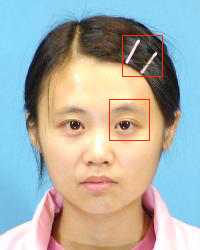
\includegraphics[width=0.23\linewidth]{img/page1_example/example_photo.png}}
\subfigure[MRF \cite{wang2009face}]{
\label{fig:example_b}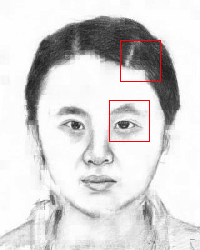
\includegraphics[width=0.23\linewidth]{img/page1_example/example_mrf.png}}
\subfigure[WMRF \cite{zhou2012markov}]{
\label{fig:example_c}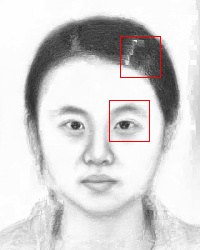
\includegraphics[width=0.23\linewidth]{img/page1_example/example_wmrf.png}}
\subfigure[SSD \cite{song2014real}]{
\label{fig:example_d}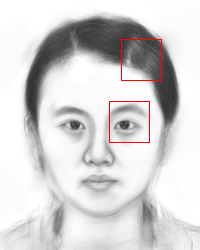
\includegraphics[width=0.23\linewidth]{img/page1_example/example_ssd.png}}
\subfigure[FCNN \cite{zhang2015end}]{
\label{fig:example_e}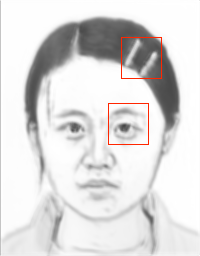
\includegraphics[width=0.23\linewidth]{img/page1_example/example_fcnn.png}}
\subfigure[BFCN \cite{zhang2017content}]{
\label{fig:example_f}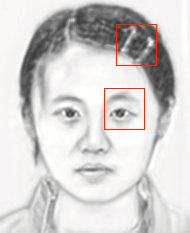
\includegraphics[width=0.23\linewidth]{img/page1_example/example_bfcn.png}}
\subfigure[\cite{gatys2015neural}$^*$]{
\label{fig:example_g}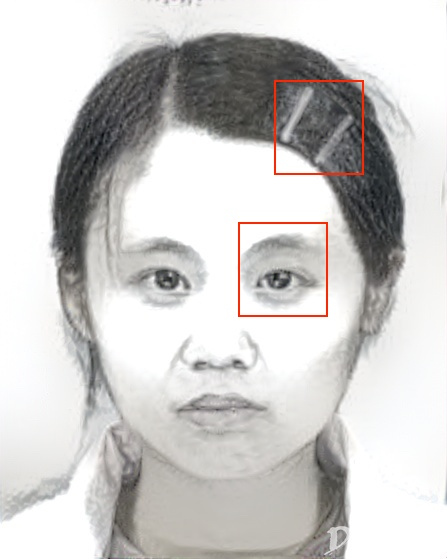
\includegraphics[width=0.23\linewidth]{img/page1_example/example_deepart.jpg}}
\subfigure[Ours]{
\label{fig:example_h}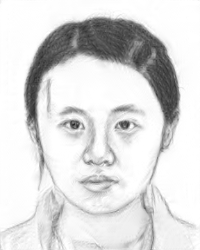
\includegraphics[width=0.23\linewidth]{img/page1_example/example_ours1.png}}

\begin{minipage}[t]{1\linewidth}
\centering
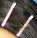
\includegraphics[width=0.11\linewidth]{img/page1_example/hairpin_photo_patch.png}
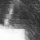
\includegraphics[width=0.11\linewidth]{img/page1_example/hairpin_mrf_patch.png}
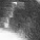
\includegraphics[width=0.11\linewidth]{img/page1_example/hairpin_wmrf_patch.png}
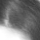
\includegraphics[width=0.11\linewidth]{img/page1_example/hairpin_ssd_patch.png}
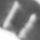
\includegraphics[width=0.11\linewidth]{img/page1_example/hairpin_fcnn_patch.png}
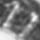
\includegraphics[width=0.11\linewidth]{img/page1_example/hairpin_bfcn_patch.png}
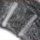
\includegraphics[width=0.11\linewidth]{img/page1_example/hairpin_deepart_patch.jpg}
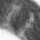
\includegraphics[width=0.11\linewidth]{img/page1_example/hairpin_ours_patch1.png}
\end{minipage}
\begin{minipage}[t]{1\linewidth}
\centering
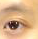
\includegraphics[width=0.11\linewidth]{img/page1_example/eye_photo.png}
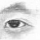
\includegraphics[width=0.11\linewidth]{img/page1_example/eye_mrf.png}
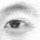
\includegraphics[width=0.11\linewidth]{img/page1_example/eye_wmrf.png}
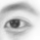
\includegraphics[width=0.11\linewidth]{img/page1_example/eye_ssd.png}
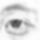
\includegraphics[width=0.11\linewidth]{img/page1_example/eye_fcnn.png}
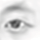
\includegraphics[width=0.11\linewidth]{img/page1_example/eye_bfcn.png}
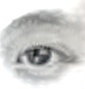
\includegraphics[width=0.11\linewidth]{img/page1_example/eye_deepart.jpg}
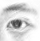
\includegraphics[width=0.11\linewidth]{img/page1_example/eye_ours1.png}
\end{minipage}
\caption[Caption for LOF]{Face sketches generated by existing methods and the proposed method. Our method can not only preserve both hair and facial content, but also contains sharp textures. %
(Note that (g) is obtained from the deep art website\setcounter{footnote}{0}\footnotemark using the photo as content and a sketch from the training set as style.)}
\label{fig:example_comp}
\end{figure}
\footnotetext{\url{https://deepart.io/}} 

Unfortunately, there exists no easy solution to face sketch synthesis due to the big stylistic gap between photos and sketches. In the past two decades, a number of exemplar based methods~\cite{wang2009face,song2014real, zhang2010lighting,zhou2012markov} were proposed. In these methods, a test photo is first divided into patches. For each test patch, a candidate sketch patch is identified by finding the most similar photo patch in a training set of photo-sketch pairs. The main drawback of this approach is that if there exists no photo patch in the training set which is  sufficiently similar to a test patch, loss of content will be observed in the synthesized sketch. For example, the sketches in the first row of Fig.~\ref{fig:example_comp} fail to keep the hairpins. Besides, some methods \cite{song2014real,zhou2012markov} blur away the textures when they try to eliminate the inconsistency between neighboring patches. Another common problem is that the synthesized sketch may not look like the test photo (see the left eye in Fig.~\ref{fig:example_b}). Recently, approaches \cite{zhang2017content,zhang2015end} based on convolutional neural network (CNN) were developed to solve these problems. Since they directly generate sketches from photos, structures and contents of the photos can be maintained. However, the pixel-wise loss functions adopted by these methods will lead to blurry artifacts (see Fig.~\ref{fig:example_e} and ~\ref{fig:example_f}) because they are incapable of preserving texture structures. The popular neural style transfer provides a better solution for texture synthesis. However, there exist two obstacles in directly applying such a technique. First, the result is easily influenced by the illumination of the photo (see the face in Fig.~\ref{fig:example_h}). Second, it requires a style image to provide the global statistics of the textures. If the given style image does not match with the target sketch (which we do not have), some side effects will occur (see the nose in Fig.~\ref{fig:example_h}). \ken{I cannot see the problem in 1(h)} %Extensive experiment and discussion is given in Section~\ref{subsec:style_transfer}. 

For an artist, the process of sketching a face usually starts with outlining the shape of the face and the key facial features like the nose, eyes, mouth and hair. Textures and shadings are then added to regions such as hair, lips, and bridge of the nose to give the sketch a specific style. Based on the above observation, and inspired by neural style transfer \cite{gatys2015texture}, we propose a new framework for face sketch synthesis from a  photo that overcomes the aforementioned limitations. In our method, a content image that outlines the face is generated by a feed-forward neural network, and textures and shadings are then added using a style transfer approach. Specifically, we design a new architecture of fully convolutional neural network (FCNN) composed of inception layers \cite{szegedy2015going} and convolution layers with batch normalization~\cite{Sergey2015batch} to generate the content image (see Section~\ref{sec:content_net}). To synthesize the textures, we first divide the target sketch into a grid. For each grid cell, we compute a newly proposed pyramid column feature using the training set (see Section~\ref{subsec:pyramid_feature_column}). A target style can then be computed from a grid of these pyramid column features, and applied to the content image. Our approach is superior to the current state-of-the-art methods in that
\begin{itemize}
\item It is capable of generating more stylistic sketches without introducing over smoothing artifacts.
\item It can preserve the content of the test photo well.
\end{itemize}

%==========================================================================
\section{Related Work}\label{sec:related_work}

\subsection{Face Sketch Synthesis}
Based on the taxonomy of previous studies~\cite{song2014real,zhou2012markov}, face sketch synthesis methods can be roughly categorized into profile sketch synthesis methods~\cite{berger2013style,chen2001example,xu2008hierarchical} and shading sketch synthesis methods~\cite{liu2005nonlinear,song2014real,tang2003face,wang2009face,zhang2015end,zhang2010lighting,zhou2012markov}. Compared with profile sketches, shading sketches are more expressive and thus more preferable in practice. Based on the assumption that there exists a linear transformation between a face photo and a face sketch, the method in~\cite{tang2003face} computes a global eigen-transformation for synthesizing a face sketch from a photo. This assumption, however, does not always hold since the modality of face photos and that of face sketches are quite different. Liu et al.~\cite{liu2005nonlinear} pointed out that the linear transformation holds better locally, and therefore they proposed a patch based method to perform sketch synthesis. In \cite{wang2009face}, a MRF based method was proposed to preserve large scale structures across sketch patches. Variants of the MRF based method were introduced in~\cite{zhang2010lighting,zhou2012markov} to improve the robustness to lighting and pose, and to render the ability of generating new sketch patches. In addition to these MRF based methods, approaches based on guided image filtering~\cite{song2014real} and feed-forward convolutional neural network~\cite{zhang2015end} are also found to be effective in transferring photos into sketches. A very recent work similar to ours is reported by Zhang \etal \cite{zhang2017content}. They proposed a two-branch FCNN to learn content and texture respectively, and then fused them through a face probability map. Although their results are impressive, their sketch textures do no look natural and the facial components are over smoothed.

%------------------------------------------------------------------------
\subsection{Style Transfer with CNN}
Texture synthesis has long been a challenging task. Traditional methods can only imitate repetitive patterns. Recently, Gatys \etal ~\cite{gatys2015texture,gatys2015neural} studied the use of CNN in style representation, and proposed a method for transferring the style of one image (referred to as the style image) to another (referred to as the content image). In their method, a target style is first computed based on features extracted from the style image using the VGG-Network. An output image is then generated by iteratively updating the content image and minimizing the difference between its style and the target style. Justin \etal \cite{feifei2016} further accelerated this process by learning a feed forward CNN in the training stage. These methods represent styles by a multi-scale Gram matrix of the feature maps. Since the Gram matrix only cares about global statistics, local structures may be destroyed when the style image is very different from the content image. Although this may not be a problem in transferring artistic styles to images, this will definitely produce noticeable artifacts in the face sketch as people are very sensitive to the distortions of the facial features. In \cite{Chen2016Patch}, Chen and Schmidt proposed a different patch based style transfer method which is better at capturing local structures. However, it is still far from satisfactory to be employed in face sketch synthesis. Our style transfer approach is inspired by but different from the above work~\cite{gatys2015texture,gatys2015neural,feifei2016} in that our target style is computed from image patches of many different images rather than from just one single image. 
\begin{figure*}[t]
\centering
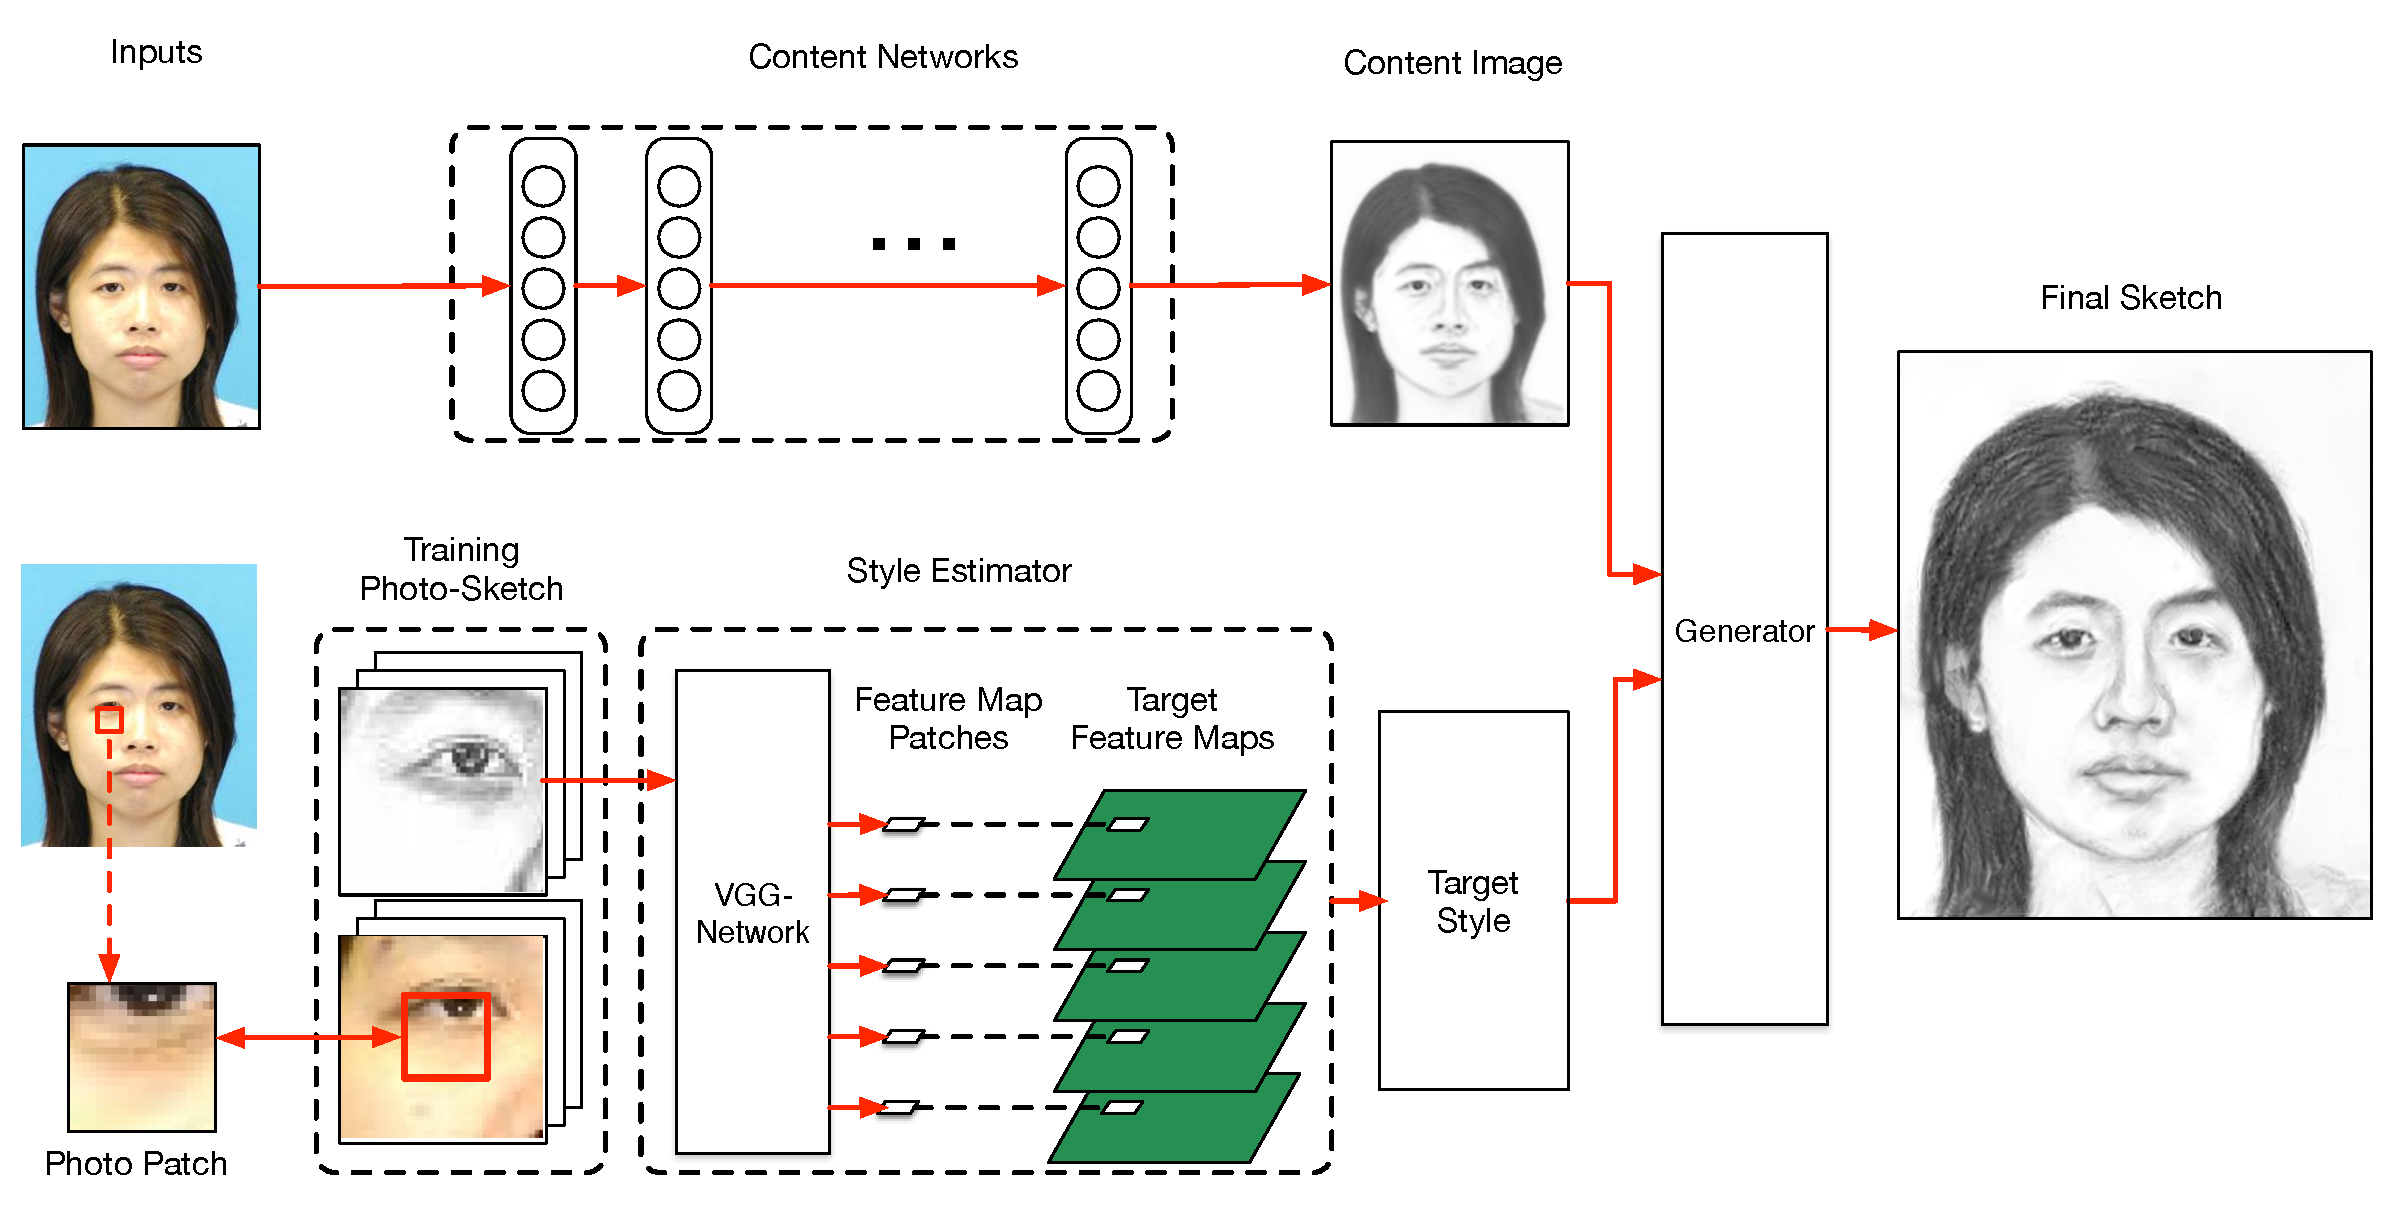
\includegraphics[width=0.85\linewidth]{img/overview.pdf}
\caption{The proposed method contains two branches which take an eye-aligned test photo as input. The content network outputs a content image which outlines the face, and the style estimator generates a target style. The final sketch is generated by combing the target style with the content image.}
\label{fig:overview}
\end{figure*}
%==========================================================================

\section{Style Representation}\label{sec:motivation}
Following the work of \cite{gatys2015neural}, we use Gram matrices of VGG-19~\cite{simonyan2014very} feature maps as our style representation. Denote the vectorized $c$th channel of the feature map in the $l$th layer of the final sketch $\mathcal{X}$ by $F^{l}_{c}(\mathcal{X})$. A Gram matrix of the feature map in the $l$th layer is then defined by the inner products between two channels of this feature map, i.e.,
\begin{equation}
G^l_{ij}(\mathcal{X}) = F^l_{i}(\mathcal{X}) \cdot F^l_{j}(\mathcal{X}), %\sum \limits_{k=1}^{M_l} F^l_{ik}(\mathcal{X}) F^l_{jk}(\mathcal{X})
\label{eq:Gram_element}
\end{equation}
where $G^l(\mathcal{X}) \in {\mathcal{R}^{N_l \times N_l}}$ %, $M_l$ is the height times width of the feature map $F^{l}(\mathcal{X})$, 
and $N_l$ is the number of channels of the feature map in the $l$th layer. Since $G^l_{ij}(\mathcal{X})$ is an inner product between two channels of the feature map, a Gram matrix is actually a summary statistics of the feature map without any spatial information. Empirically , a Gram matrix of the feature map captures the density distribution of a sketch. For example, if a given style (sketch) image has much less hair than the test photo, the synthesized sketch $\mathcal{X}$ will become brighter than a natural sketch (see experimental results in Section~\ref{subsec:style_transfer}). Thus it is important to have a style (sketch) image which is (statistically) similar to the test photo. Note that, in face sketch synthesis, however, there usually does not exist a single photo-sketch pair in the training set that matches all properties of the test photo. How to compute a target style for the synthesized sketch $\mathcal{X}$ is therefore not trivial, and is the key to the success of this approach. We will introduce a feature-space patch-based approach to solve this problem in Section~\ref{subsec:pyramid_feature_column}.
%. We hence propose a feature level patch based method to estimate the style of the final sketch. Each feature patch corresponds to a sketch patch. The reason why we can separate features into patches comes from \cite{Li2017Demistify}. The feature vectors at different position of feature map can be viewed as independent samples when we use gram matrix. 

%==========================================================================
\section{Methodology}
Our method can be classified as a shading synthesis method. The steps of our method are summarized in Fig.~\ref{fig:overview}. First, a preprocessing step as described in~\cite{wang2009face} is carried out to align all photos and sketches in the training set by the centers of the two eyes. An eye-aligned test photo $\mathcal{I}$ is then fed into two branches, namely the content network and the style estimator. The content network converts $\mathcal{I}$ into a content image $\mathcal{C}$, which outlines the shape of the face and the key facial features such as nose, eyes, mouth and hair. The style estimator divides $\mathcal{I}$ into a grid of non-overlapping $16\times16$ patches. For each test patch, it locates the most similar photo patch from the photo-sketch pairs in the training set and produce a target sketch patch from the corresponding sketch in the pair. A pyramid column feature (Section~\ref{subsec:pyramid_feature_column}) is then computed for the target sketch patch. Finally, a target style can be computed from a grid of these pyramid column features, and a final sketch $\mathcal{X}$ can be synthesized by applying the target style to $\mathcal{C}$ through neural style transfer~\cite{gatys2015neural}. 
% takes a $16\times16$ local patch from test photo as input and searches photo-sketch pairs in the training set to find a target sketch patch $S_{ij}$ ($(i, j)$ denotes the patch location). Each  $S_{ij}$ with its surrounding region can generate a pyramid feature column $U_{ij}$. Combining all $U_{ij}$, we can get the target style features of $\mathcal{I}$, \ie $\tilde{U}$. Given $\mathcal{C}$ and $\tilde{U}$, we can generate a sketch $\mathcal{X}$ that combines the content information in $\mathcal{C}$ with the style representation $\tilde{U}$ following the iterative procedure in \cite{gatys2015neural}. 

%------------------------------------------------------------------------
\subsection{Content Image Generation} \label{sec:content_net}
\begin{figure*}[htbp]
\centering
\subfigure[The architecture of content network]{
\label{fig:content_NN_a}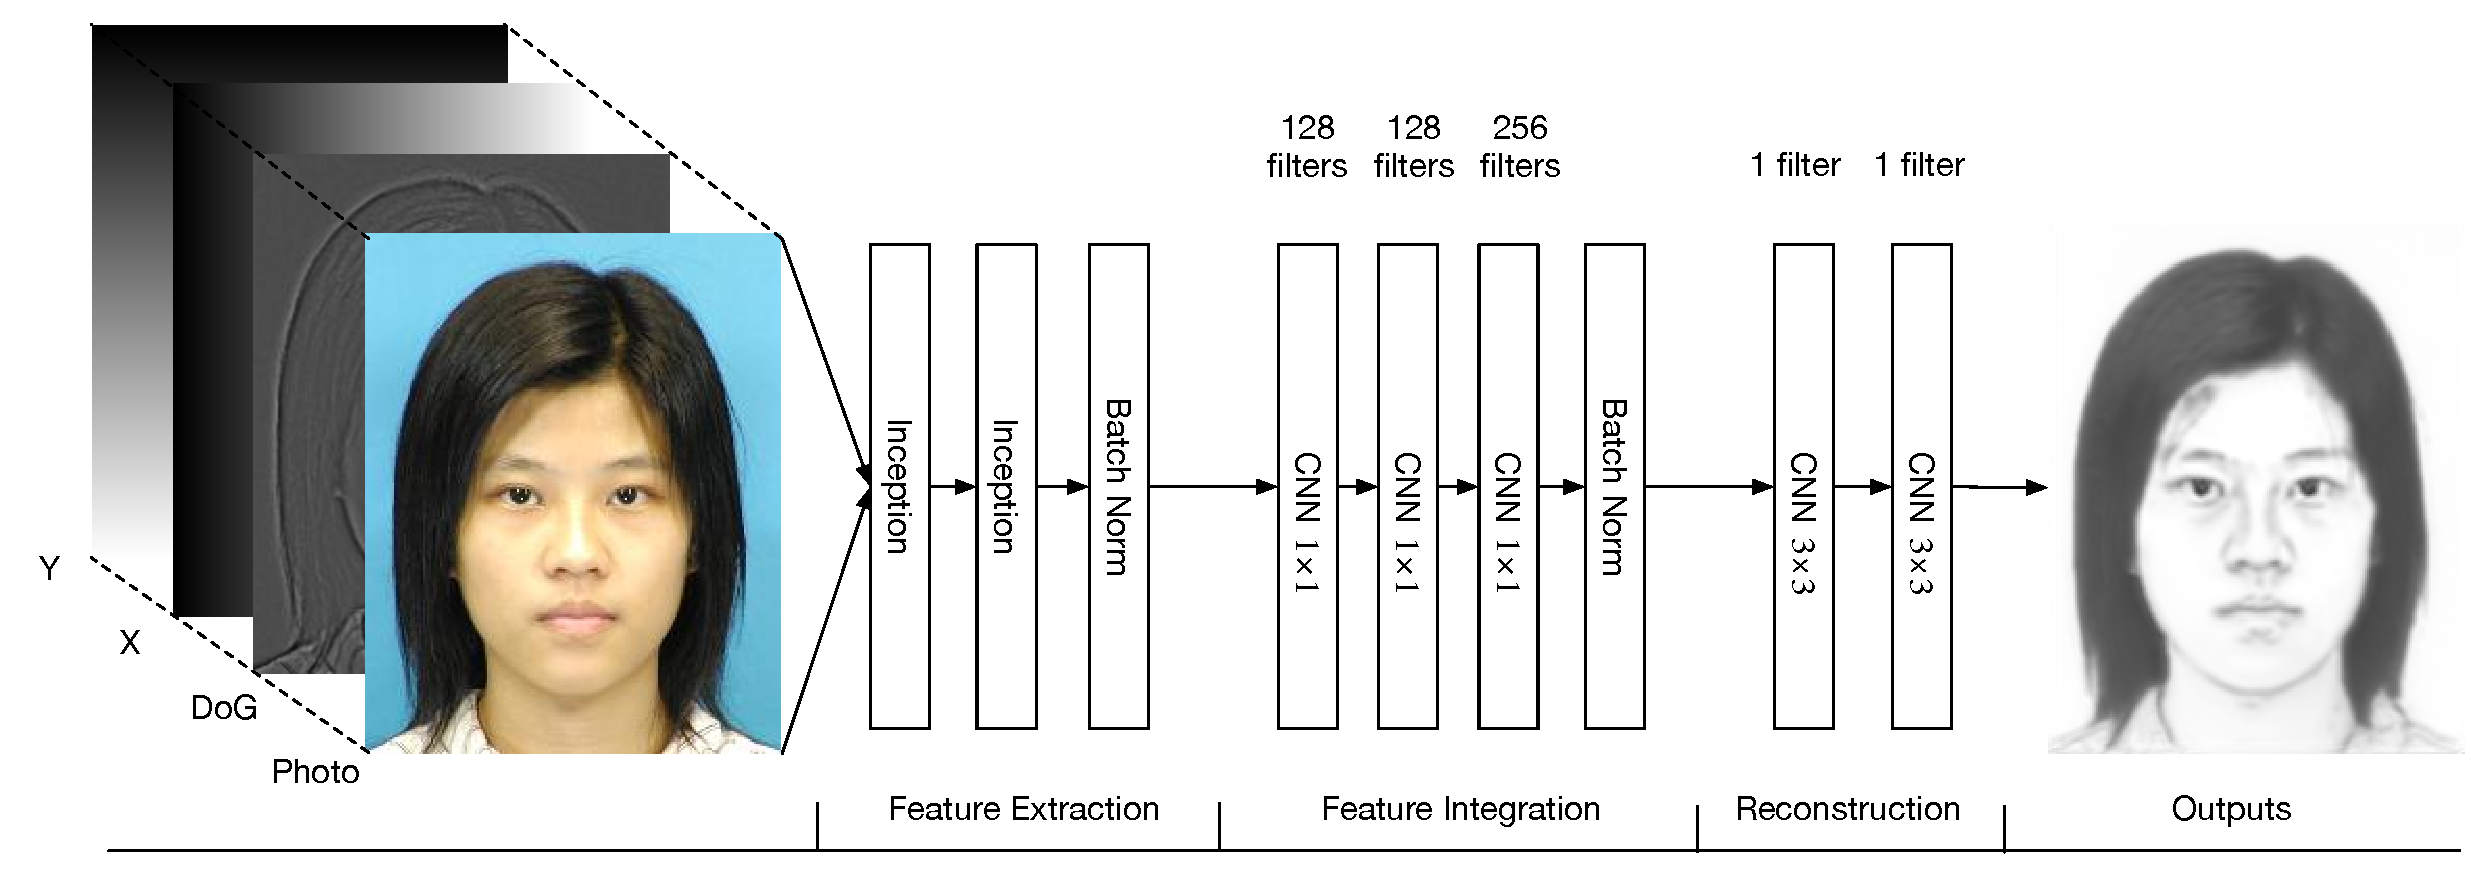
\includegraphics[width=0.65\linewidth]{img/content_net.pdf}}
\subfigure[Inception module]{
\label{fig:content_NN_b}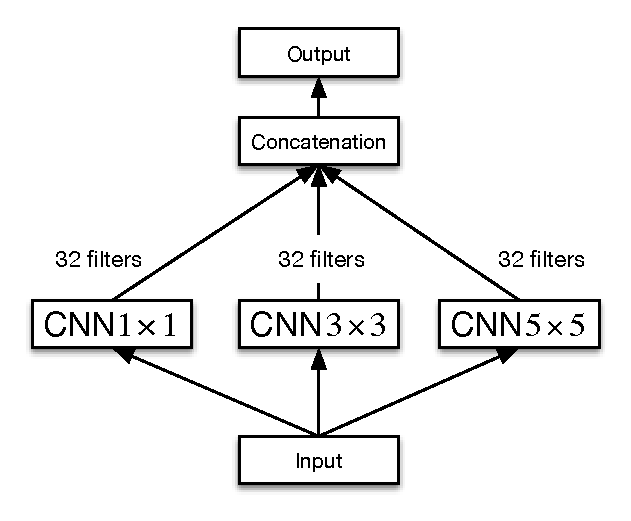
\includegraphics[width=0.25\linewidth]{img/inception.pdf}}
\caption{Illustration of the content network for generating a content image. The numbers above the building block denote the number of CNN filters. (a) The architecture of content network. (b) The inception module in (a) contains three groups of filters with different sizes.}
\label{fig:content_NN}
\end{figure*}

The architecture of our content network is shown in Fig.~\ref{fig:content_NN}. Besides the test photo, we feed three extra channels containing the spatial information (i.e., $x$ and $y$ coordinates) and a difference of Gaussian (DoG) image into our content network. As pointed out in \cite{wang2009face}, face sketch synthesis algorithms can benefit from integrating features from multiple resolutions. Hence, we employ an inception module %inspired by the GoogLeNet~
\cite{szegedy2015going} for feature extraction, which concatenates features generated from three groups of filters %with different spatial resolutions. Our inception unit contains 3 different size of filters
with a size of $1\times1$, $3\times3$ and $5\times5$ respectively (see Fig.~\ref{fig:content_NN_b}). Features extracted using a two-layer-inception module are then fed into a three-layer-CNN for feature integration, where all filters have a size of $1\times1$. Finally, the integrated features are used to reconstruct the content image $\mathcal{C}$  by a two-layer-CNN with the filter size being $3\times3$. Since $L_1$-norm is better at preserving details than $L_2$-norm, we use the $L_1$-norm between $\mathcal{C}$ and the ground truth sketch $S$ as the loss function in training our content network, i.e.,
\begin{equation}
\mathcal{L}_s = \frac{1}{N} \sum \limits_{i=1}^N \|\mathcal{C}_i - S_i\| \label{eq:content-net-loss}
\end{equation}
where $N$ is the number of training photos. 

\subsection{Style Estimation} \label{subsec:pyramid_feature_column}
%------------------------------------------------------------------------
As mentioned previously, there usually does not exist a single photo-sketch pair in the training set that matches all properties of the test photo. In order to estimate a target style for the final sketch $\mathcal{X}$, we subdivide the test photo into a grid of non-overlapping $16\times16$ patches. For each test patch, similar to previous work  \cite{wang2009face,zhou2012markov}, we find the best matching photo patch from the photo-sketch pairs in the training set in terms of MSE \ken{defines MSE}. A target sketch patch can then be obtained from the corresponding sketch in the photo-sketch pair containing the best matching photo patch. Instead of compositing a style image using the thus obtained target sketch patches, which may show inconsistency across neighboring patches, we adopt a feature-space approach here. We extract feature patches from the feature maps of the original sketch at 5 different layers of the VGG-Network, namely $conv1\_1$, $conv2\_1$, $conv3\_1$, $conv4\_1$ and $conv5\_1$ respectively, that correspond to the target sketch patch. These feature patches have a size of $16\times16$, $8\times8$, $4\times4$, $2\times2$ and $1\times1$ respectively (see Fig.~\ref{fig:pyramidcolumn}). We group these five feature patches of a target sketch patch and call it a  {\em pyramid column feature}. Finally, a target style, in the form of Gram matrices, can be computed directly from a grid of such pyramid column features.

%Fig. \ref{fig:pyramidcolumn} shows an example of the pyramid feature column. Denote the feature maps (of the $l$th layer) used to estimate the style of the final sketch by $A^{l}$. In our feature patch based method, we divide $A^{l}$ into a fixed size of grid. Due to the different feature map size, the sizes of the feature patches at layer $conv1\_1$, $conv2\_1$, $conv3\_1$, $conv4\_1$ and $conv5\_1$ are $16\times16$, $8\times8$, $4\times4$, $2\times2$ and $1\times1$. The photos and sketches are resized to $288\times288$, thus the size of grid is $18\times18$. Grouping feature map patches having the same grid indexes $(i, j)$ at different layers together, we get a pyramid feature column $U_{ij}$. To estimate $U_{ij}$, a sketch patch in the training set is fed to the VGG-Network and a pyramid column is composed of the resulting feature maps. This process consists of two steps: (1) find a matching sketch patch $S_{ij}$ from the training set for $U_{ij}$ and (2) feed $S_{ij}$ to VGG-Network and extract $U_{ij}$ from the resulting feature maps.

\begin{figure}[htbp]
\centering
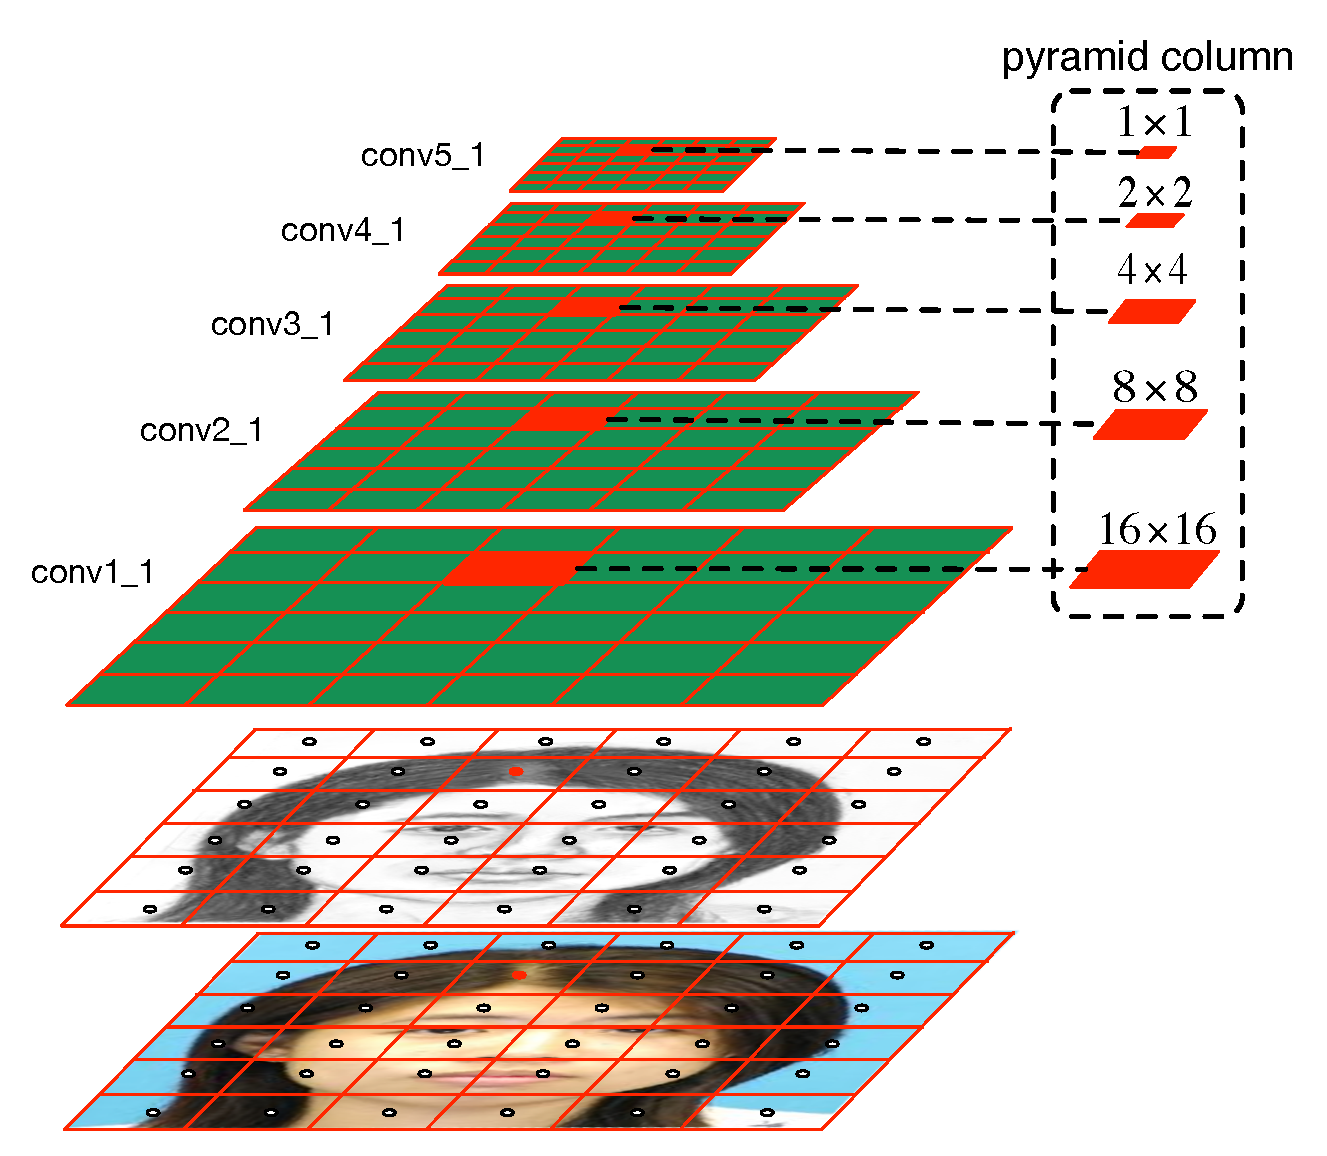
\includegraphics[width=0.85\linewidth]{img/pyramidcolumn.pdf}
\caption{Illustration of the pyramid column feature. \ken{rewrite this caption}}
\label{fig:pyramidcolumn}
\end{figure}

%\paragraph*{Find Matching Sketch Patch} Similar to previous works~\cite{wang2009face,zhou2012markov}, we examine the similarity of test photo patch and train photo patches to find a matching sketch $S_{ij}$ for $U_{ij}$. Denote the train photo patch set as $P$, given a test photo patch $T'_{ij}$, the target sketch patch $S_{ij}$ is found by
%\begin{gather}
%S_{ij} = \phi(\min_{T^k_{mn} \in P} f(T^k_{mn}, T'_{ij})) \\
%m = i + \Delta x, n = j + \Delta y
%\end{gather}
%where $T^k_{mn}$ is the photo patch of the $k$th image at $(m, n)$ in training set, $\phi$ is a one-to-one mapping between photo patch and sketch patch, $\Delta x$ and $\Delta y$ is the shift of $(m, n)$ around $(i, j)$. The function $f$ measures the discrepancy between $T^k_{mn}$ and $T'_{ij}$. Because we only need the test photo patch and train photo patch have a similar appearance, we simply use MSE as $f$ here.

%\paragraph*{Estimate Pyramid Feature Column}
%After we get $S_{ij}$, we can compute the corresponding pyramid feature column $U_{ij}$. Although the feature column can be generated by a $16\times16$ patch, padding zeros is not a good idea. Therefore, we will make use of the surrounding area of $S_{ij}$ to compute $U_{ij}$. According to the architecture of VGG-19, the receptive field of $conv5\_1$ is 132 without padding. To get $16\times16$ patches, we will need a $144\times144$ region $\mathcal{R}$ containing 81 patches in total. $S_{ij}$ should be at the center of $\mathcal{R}$, \ie $S_{55}$ with respect to the grids of $\mathcal{R}$. For those border part where we can't find a region centered at $S_{ij}$, we just find another region $\mathcal{R}'$ which has the biggest intersection with the should be region $\mathcal{R}$ (the blue box in Fig. \ref{fig:border_example}). The $S_{55}$ in $\mathcal{R}$  should be $S'_{pq}$ in $\mathcal{R}'$ ($(p, q)$ is calculated according to different conditions). The feature column $U_{55}$ in $\mathcal{R}$ or $U_{pq}$ in $\mathcal{R'}$ is the estimated pyramid feature column. 

%Allocating all these feature columns to its original patch location $(i, j)$, we can get the final feature maps $\tilde{U}$ and use it to compute gram matrix.  

%\begin{figure}[htbp]
%\centering
%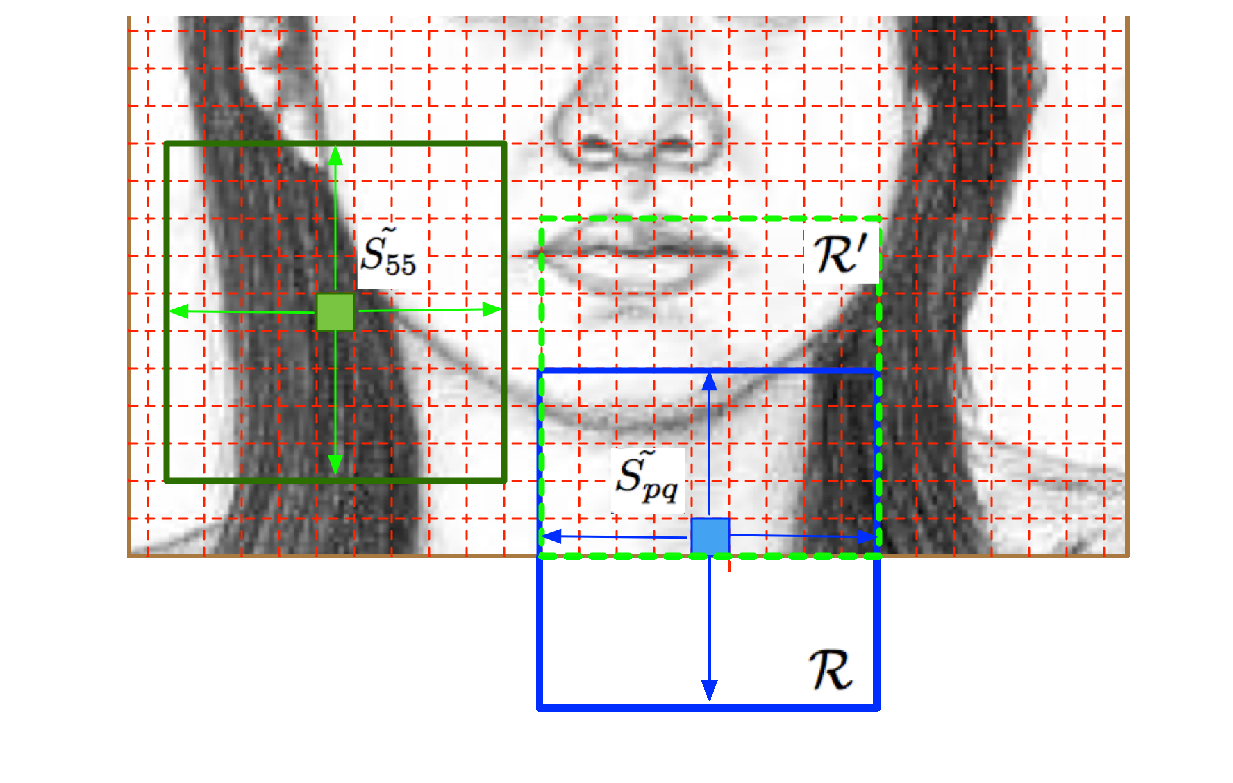
\includegraphics[width=0.99\linewidth]{img/border_PFC.eps}
%\caption{Find a region $\mathcal{R}$ centered at $S_{ij}$. If $\mathcal{R}$ is inside the image, $S_{ij}$ should be the center patch of $\mathcal{R}$, see the left region. Otherwise, we need to find $\mathcal{R}'$ inside the image which has the biggest intersection with $\mathcal{R}$, see the right part. Suppose the indexes of $\tilde{S_{ij}}$ inside $\mathcal{R}'$ is $(p, q)$, then $U_{pq}$ is the corresponding feature column.}
%\label{fig:border_example}
%\end{figure}

\subsection{Loss Function for Sketch Generation}

Similar to \cite{gatys2015neural}, our loss function is composed of a content loss and a style loss. In addition, we introduce a component loss to enhance the key facial components. The total loss is

\begin{equation}
\mathcal{L}_{t}( \mathcal{X} ) = \alpha \mathcal{L}_{c} + \beta_1 \mathcal{L}_{s} + \beta_2 \mathcal{L}_{k},
\label{eq:Total_loss}
\end{equation}
where $\alpha$, $\beta$ and $\beta_2$ are the weights for the different loss terms.
We minimize the loss function by updating the target sketch $\mathcal{X}$ \redn[without changing the VGG parameters(?)].

The content loss is defined by the difference between the feature map at layer conv1\_1 of the synthesized sketch and that of the content image :
\begin{equation}
\mathcal{L}_{c}( \mathcal{X} ) = \| {{F^{\rm{conv1\_1}}}( \mathcal{X} ) - {F^{\rm{conv1\_1}}}( \mathcal{C} )} \|_2^2.
\label{eq:content_loss}
\end{equation}
The style loss is defined by the difference between the Gram matrices of the synthesized sketch and that of the target style:
\begin{equation}
\mathcal{L}_{s} ( \mathcal{X} ) = \sum\limits_{l \in {L_s}} {\frac{1}{{M_l^2N_l^2}}\| {{G^l}(\mathcal{X} ) - G^l(\mathcal(T))} \|_2^2} 
\label{eq:Gram_loss}
\end{equation}
where $N_l$ denotes the number of channels of the feature map at layer $l$, and $M_l$ is the product of width and height of the feature map at layer $l$, and $G^l(\mathcal{T})$ is the Gram matrix computed from the grid of pyramid column features.  

To better transfer styles of the key facial components, we employ a component loss to encourage the key component style of the final sketch to be the same as the target key component style. Since all photos and sketches have been aligned by the centers of the two eyes, the key components lie roughly within a rectangular region $\mathcal{R}$ with the eyes positioned at its upper corners. Here, we define the key component style by Gram matrices computed from feature maps corresponding to  the rectangular region $\mathcal{R}$. The component loss is defined as
\begin{equation}
\mathcal{L}_{k} ( \mathcal{X} ) = \sum\limits_{l \in {L_s}} {\frac{1}{{\hat{M}_l^2{N}_l^2}}\| {{{\hat G}^l}( \mathcal{X} ) - {\hat G}^l(\mathcal{T})} \|_2^2} 
\label{eq:component_loss}
\end{equation}
where $\hat G^l$ denotes the Gram matrix computed for the rectangular region $\mathcal R$, and $\hat{M}_l$ is the product of width and height of the feature map at layer $l$ corresponding to $\mathcal R$. 

%------------------------------------------------------------------------
\subsection{Implementation Details}

\paragraph*{VGG-19 Parameters} Since the VGG-Network is originally designed for color images, while sketches are gray scale images, we modify the first layer of VGG-Network for gray scale images by setting the filter weights to
\begin{equation}
W^{k} = W^{k}_r+W^{k}_g+W^{k}_b
\label{eq:VGG_weights}
\end{equation}
where $W^{k}_r$, $W^{k}_g$, and $W^{k}_b$ are weights of the $k$th filter in the first convolutional layer for the R, G and B channels respectively, and $W^{k}$ is the weight of the $k$th filter in the first convolutional layer of our modified network.

\paragraph{Data Partition} CUHK \ken{ref?} has 88 training photos and 100 test photos, and AR \ken{ref?} has 123 photos. Our training set is composed of the 88 training photos of CUHK and 100 photos from AR. When training the content network, 10\% of the training set are taken out as the validation set. All the 188 photo-sketch pairs are used to generate target sketch.

\paragraph{Training the Content Network} The input photo-sketch pairs are all resized to $200\times256$ \ken{not $288\times288$?} and aligned by the centers of the two eyes. A mirror padding is carried out before the convolution operation when necessary to ensure the output feature map is of the same size as the input \ken{?}. Adadelta \cite{matt2012adadelta} is used as the optimizer because it is stable and much faster than others.  

\paragraph{Sketch Generation} 
In all experiments, we resize the test photos and the photo-sketch pairs in the training set to $288\times288$. The final sketch is obtained by resizing the resulting sketch back to the original size. The size of $\mathcal{R}$ is $48\times48$. The weights in Eq.~(\ref{eq:Total_loss}) are $\alpha=0.004$, $\beta_1=1$ and $\beta_2=0.1$. The minimization is carried out using L-BFGS. Instead of using random noises, we use the content image as a starting point, which will make the optimization process converge much faster. 

%==========================================================================

\begin{figure*}[htbp]
\centering
\subfigure[Photo]{
\begin{minipage}[b]{0.1\linewidth}
\centering
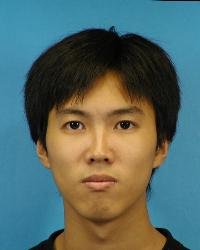
\includegraphics[width=0.91\linewidth]{img/sketch_result/photo1.png}
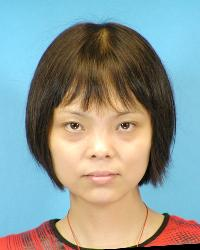
\includegraphics[width=0.91\linewidth]{img/sketch_result/photo2.png}
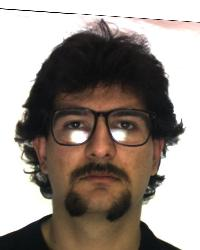
\includegraphics[width=0.91\linewidth]{img/sketch_result/photo3.png}
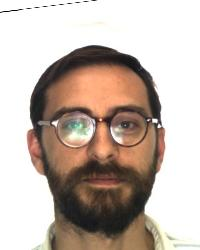
\includegraphics[width=0.91\linewidth]{img/sketch_result/photo4.png}
\end{minipage}
}
\subfigure[MRF]{
\begin{minipage}[b]{0.13\linewidth}
\centering
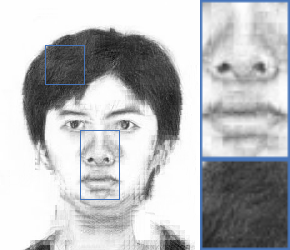
\includegraphics[width=0.99\linewidth]{img/sketch_result/mrf_s1.png}
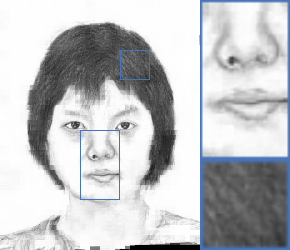
\includegraphics[width=0.99\linewidth]{img/sketch_result/mrf_s2.png}
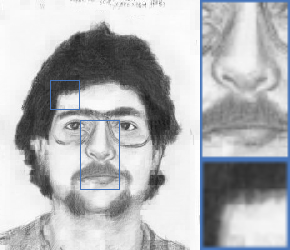
\includegraphics[width=0.99\linewidth]{img/sketch_result/mrf_s3.png}
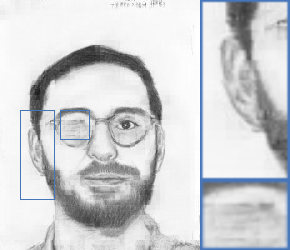
\includegraphics[width=0.99\linewidth]{img/sketch_result/mrf_s4.png}
\end{minipage}
}
\subfigure[WMRF]{
\begin{minipage}[b]{0.13\linewidth}
\centering
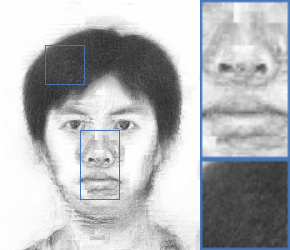
\includegraphics[width=0.99\linewidth]{img/sketch_result/mwf_s1.png}
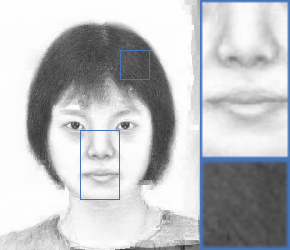
\includegraphics[width=0.99\linewidth]{img/sketch_result/mwf_s2.png}
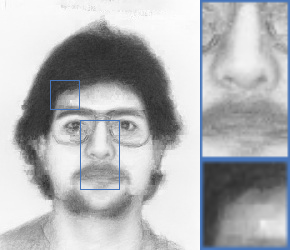
\includegraphics[width=0.99\linewidth]{img/sketch_result/mwf_s3.png}
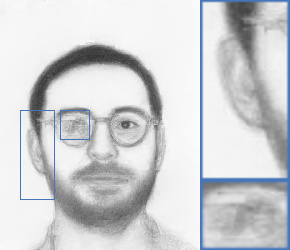
\includegraphics[width=0.99\linewidth]{img/sketch_result/mwf_s4.png}
\end{minipage}
}
\subfigure[SSD]{
\begin{minipage}[b]{0.13\linewidth}
\centering
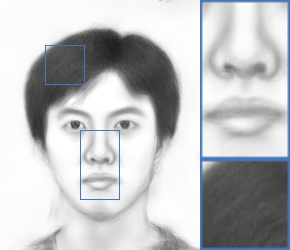
\includegraphics[width=0.99\linewidth]{img/sketch_result/ssd_s1.png}
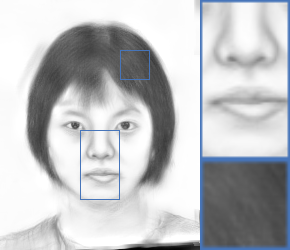
\includegraphics[width=0.99\linewidth]{img/sketch_result/ssd_s2.png}
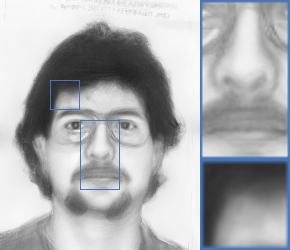
\includegraphics[width=0.99\linewidth]{img/sketch_result/ssd_s3.png}
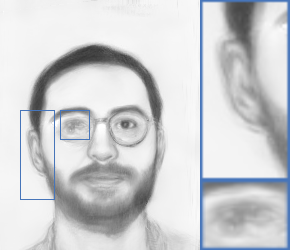
\includegraphics[width=0.99\linewidth]{img/sketch_result/ssd_s4.png}
\end{minipage}
}
\subfigure[FCNN]{
\begin{minipage}[b]{0.13\linewidth}
\centering
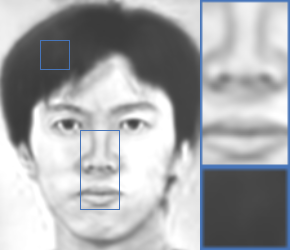
\includegraphics[width=0.99\linewidth]{img/sketch_result/fcnn_s1.png}
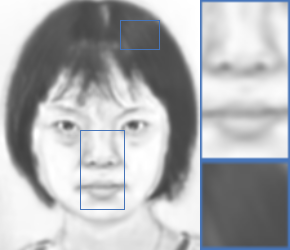
\includegraphics[width=0.99\linewidth]{img/sketch_result/fcnn_s2.png}
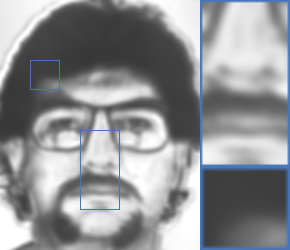
\includegraphics[width=0.99\linewidth]{img/sketch_result/fcnn_s3.png}
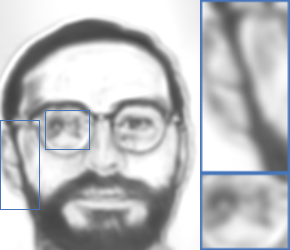
\includegraphics[width=0.99\linewidth]{img/sketch_result/fcnn_s4.png}
\end{minipage}
}
\subfigure[BFCN]{
\begin{minipage}[b]{0.13\linewidth}
\centering
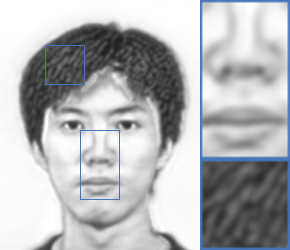
\includegraphics[width=0.99\linewidth]{img/sketch_result/bfcn_s1.png}
\includegraphics[width=0.99\linewidth]{img/sketch_result/bfcn_s2.png}
\includegraphics[width=0.99\linewidth]{img/sketch_result/bfcn_s3.png}
\includegraphics[width=0.99\linewidth]{img/sketch_result/bfcn_s4.png}
\end{minipage}
}
\subfigure[Ours]{
\begin{minipage}[b]{0.13\linewidth}
\centering
\includegraphics[width=0.99\linewidth]{img/sketch_result/ours_s1.png}
\includegraphics[width=0.99\linewidth]{img/sketch_result/ours_s2.png}
\includegraphics[width=0.99\linewidth]{img/sketch_result/ours_s3.png}
\includegraphics[width=0.99\linewidth]{img/sketch_result/ours_s4.png}
\end{minipage}
}
% \includegraphics[width=0.99\linewidth]{img/sketch_result/sketch_result_draft.pdf}
\caption{Examples of qualitative evaluation on CUHK (first two rows) and AR (last two rows). (a) The sketches drawn by artists. (b) MRF~\cite{wang2009face} (c) WMRF~\cite{zhou2012markov} (d) SSD~\cite{song2014real} (e) FCNN~\cite{zhang2015end} (f) BFCN~\cite{zhang2017content} (g) Ours. The proposed method preserves more texture details, for example in the hair and nose. It is also best at keeping the origin structures of photos, such as the glasses.}
\label{fig:qua_eval}
\end{figure*}

\section{Experiments}

We evaluate the performance of the proposed method against other state-of-the-art methods on the CUHK student dataset~\cite{wang2009face} and the AR dataset~\cite{martinez1998r}. We compare the results of our method against other 6 methods including traditional approaches and recent deep learning models. After discussing the disadvantages of previous quantitative evaluation criteria, we introduce the Normalized Gram Matrix Difference (NGMD) as a new evaluation tool. We believe that NGMD is more effective and will greatly promote the sketch qualities in future work.

%------------------------------------------------------------------------
\subsection{Style Transfer Evaluation} \label{subsec:style_transfer}

Although style transfer has shown remarkable performance in artistic style, it can't be directly applied to face sketch synthesis, see Fig.~\ref{fig:example_h}. The generated sketch is greatly influenced by illumination of original photo and doesn't look like sketch at all. To prove our assumption in Section~\ref{sec:motivation} that gram matrix captures the density distribution of sketch, we replace the original RGB photo with content image generated by our content network. We selected 3 sketch styles with different amount of hairs and see how it influences the result. Fig.~\ref{fig:style_result} shows a clear relationship between the hair amount of sketch and pixel intensities of sketch result. The facial key parts in Fig.~\ref{fig:style_result2} and \ref{fig:style_result3} are missed. Therefore, even with a content structure, the original style transfer is still not suitable for elaborate task. However, if the style image has a similar structure with test photo, for example Fig.~\ref{fig:style_result1}, the results can be quite good. This inspires our feature patch based method. Image patch method is not considered because it will introduce patch inconsistency as discussed in Section~\ref{sec:related_work}. 

\begin{figure}[htbp]
\centering
\subfigure[]{
\label{fig:style_content} \includegraphics[width=0.23\linewidth]{img/style_evaluate/content.png}}
\subfigure[]{
\label{fig:style_result1} \includegraphics[width=0.23\linewidth]{img/style_evaluate/style_result1.pdf}}
\subfigure[]{
\label{fig:style_result2} \includegraphics[width=0.23\linewidth]{img/style_evaluate/style_result2.pdf}}
\subfigure[]{
\label{fig:style_result3} \includegraphics[width=0.23\linewidth]{img/style_evaluate/style_result3.pdf}}
\caption{(a) is the content image generated by our content network. (b), (c) and (d) are generated by different styles. It can be seen that when the hair decreases the generated sketch becomes brighter.}
\label{fig:style_result}
\end{figure}

%------------------------------------------------------------------------
\subsection{Sketch Generation} \label{sec:sketch_gen}

Fig.~\ref{fig:qua_eval} shows the comparison between our methods and many other approaches. The first two rows are from CUHK test set, and the last two are from AR. We can see that our method can generate more stylistic sketches than others. For example, in the hair part, only MRF, BFCN and the proposed method can generate obvious textures. However, the texture of MRF is not continuous in the border part and introduce many other artifacts, and the texture of BFCN doesn't look like human strokes. Both WMRF and SSD introduce over smoothing effect and FCNN is not able to give clear textures. Our method can not only generate textures for hairs and mustache but also shadings, for example the nose part.

On the other hand, only BFCN and the proposed method can handle structures decorated on the face well, for example the glasses of the last two row. MRF, WMRF and SSD are exemplar based method so they can't handle something different from training set, the glass edges of them are not complete. FCNN, BFCN and our method generate the image content by CNN, so they can handle the original photo structures well. But both FCNN and BFCN care nothing about the textures of facial part, so their results are not good considering the face part. In contrast, our method can well maintain the image content and attach textures similar to human paintings. 

%------------------------------------------------------------------------
\subsection{Quantitative Results}

\begin{table}[htbp]
\small
\begin{tabular}{C{0.2cm}C{0.2cm}C{0.2cm}C{0.1cm}C{0.3cm}C{0.1cm}C{0.35cm}C{0.1cm}C{0.35cm}C{0.1cm}C{0.1cm}C{0.1cm}C{0.25cm}}
\hline
\multicolumn{2}{c|}{\multirow {2}{*}{Methods}} & \multicolumn{5}{c}{AR} & & \multicolumn{5}{c}{CUHK} \\
\cline{3-7} \cline{9-13} \multicolumn{2}{c|}{} & R1 & & R5 & & R10 & & R1 & & R5 & & R10   \\
\hline
\multicolumn{2}{c|}{FCNN} & - & & - & & - & & 81\% & & 96\% & & 97\%   \\
\multicolumn{2}{c|}{MRF}  & 97.5\% & & 97.5\% & & \textcolor{red}{100\%} & & 83\% & & 96\% & & 96\% \\
\multicolumn{2}{c|}{WMRF} & 97.5\% & & 97.5\% & & \textcolor{red}{100\%} & & 83\% & & 97\% & & 98\%  \\
\multicolumn{2}{c|}{SSD}  & 96.7\% & & 97.5\% & & \textcolor{red}{100\%} & & \textcolor{red}{87\%} & & 97\% & & 98\%   \\
\multicolumn{2}{c|}{Ours} & \textcolor{red} {98.4\%} & & \textcolor{red} {98.4\%} & & \textcolor{red} {100\%} & & \textcolor{red} {87\%} & & \textcolor{red} {98\%} & & \textcolor{red} {99\%}   \\
\hline
\end{tabular}
\caption{Recognition rate on benchmark datasets. The best performance is colored in red.}
\label{tab:reg_percentage}
\end{table}

\begin{table*}[htbp]
\begin{center}
{\small
\begin{tabular}{ccccccccccccc}
\hline
\multicolumn{2}{c|}{\multirow {2}{*}{Methods}} &\multicolumn{5}{c}{AR} & & \multicolumn{5}{c}{CUHK} \\
\cline{3-7} \cline{9-13} \multicolumn{2}{c|}{} & conv1\_1 & conv2\_1 & conv3\_1 & conv4\_1 & conv5\_1 & &
 conv1\_1 & conv2\_1 & conv3\_1 & conv4\_1 & conv5\_1  \\
\hline
\multicolumn{2}{c|}{FCNN} & - & - & - & - & - & & { $0.009$} &{ $0.110$} & {$0.080$} & {$9.43$} & {$1.49$}  \\
\multicolumn{2}{c|}{MRF} & 0.0043 & 0.009 & {$0.033$}  & {$0.12$} & 0.28 & & { $0.010$} &{ $0.014$} & {$0.047$} & $0.13$ & $0.18$  \\
\multicolumn{2}{c|}{WMRF} & 0.0053 & 0.027 & {$0.085$}  & {$0.19$} & 0.29 & & { $0.010$} &{ $0.052$} & {$0.052$} & {$0.27$} & {$0.19$}  \\
\multicolumn{2}{c|}{SSD} & 0.0056 & 0.036 & {$0.110$} & {$1.90$} & 0.28 & & { $0.009$} &{ $0.102$} & {$0.070$} & {$3.32$} & {$0.24$}  \\
\multicolumn{2}{c|}{Ours} & {\color{red} 0.0035} & {\color{red} 0.008} & {\color{red} $0.029$} & {\color{red} $0.08$} & {\color{red} $0.17$} & & {\color{red}$0.007$} &{\color{red} $0.012$} & {\color{red} $0.033$} & {\color{red} $0.07$} & {\color{red} $0.12$}  \\
\hline
\end{tabular}
}
\end{center}
\caption{Averaged NGMD value of different methods at different level on AR and CUHK datasets. A smaller NGMD indicates the generated texture is more similar to ground truth.}
\label{tab:NGMD}
\end{table*}

\paragraph*{Sketch Recognition} Sketch synthesis methods are usually evaluated quantitatively  via the face sketch recognition task~\cite{song2014real,wang2009face,zhang2015end,zhou2012markov}. If an algorithm achieves higher sketch recognition rates, it suggests that this method is more effective in synthesizing sketches. We adopt the widely used PCA based recognition method with ``rank-1 (R1)'', ``rank-5 (R5)'' and ``rank-10 (R10)'' criteria ~\cite{wang2009face} where ``rank $n$'' measures the rate of the correct answer in the top $n$ best matches. The results of different methods are shown in Table~\ref{tab:reg_percentage}. Our method achieves the best performance against all other methods in the ``R1'' and ``R5'' tests. 

However, such kind of evaluation is not effective since every one is close to 100\%, and more importantly, it can't guide our research effort. Zhang \etal \cite{zhang2015end} proposed a  Multiscale Pixel-wise Reconstruction Loss (MPRL). Although we agree that if MPRL is zero, the generated sketches will be exactly the same with ground truth, there are two reasons why it is not a good criteria. First, experiment results of \cite{zhang2015end, zhang2017content} show that $L_2$-norm would give blurry sketches. Second, the ground truth draw by human usually doesn't correspond exactly with photos, thus difficult for algorithms to reach the ground truth.

Meanwhile, human can often be able to tell whether a sketch is generated by algorithms or drawn by artists just from a quick glance without examining details.
This indicates that there exists a big gap between the style of algorithm-generated sketches and that of those drawn by artists. And we need a criteria which can quantitatively measure such gap.

\paragraph*{Normalized Gram Matrix Difference (NGMD)} To quantitatively evaluate the style similarity between a generated sketch and the sketch drawn by a real artist, we employ the normalized gram matrix difference (NGMD) between the generated sketch $\mathcal{X}$ and the drawn sketch ${\tilde {\mathcal{X}}}$:
\begin{equation}
{D^l_s}\left( {\mathcal{X},\tilde {\mathcal{X}}} \right) = \frac{{\left\| {{G^l}\left( \mathcal{X} \right) - {G^l}\left( {\tilde {\mathcal{X}}} \right)} \right\|_2^2}}{{\left\| {{G^l}\left( {\tilde {\mathcal{X}}} \right)} \right\|_2^2}}
\label{eq:style_exp}
\end{equation}
where $l\in L_s$. The smaller the NGMD value is, the more similar $\mathcal{X}$ and ${\tilde {\mathcal{X}}}$ are. 

It is exciting how well NGMD match our intuition, see Fig.~\ref{fig:qua_eval}. 
The results of~\cite{zhang2015end} can roughly outline the sketches but can't add textures, thus they got a high NGMD in Table~\ref{tab:NGMD}. The results of MRF~\cite{wang2009face} and WMRF~\cite{zhou2012markov} are more similar to hand drawn sketches in style since these exemplar based approaches use patches of hand drawn sketches to make up the target sketch. That is why they have a smaller NGMD value. Inheriting the ability of denoising, the filtering based approach~\cite{song2014real} is good at suppressing noises in the results. However, it is also likely for this method to over-smooth the results, which will deteriorate the texture, thus its NGMD value is higher than WMRF. 

%------------------------------------------------------------------------
\subsection{Generalization Evaluation}

\begin{figure}[htbp]
\centering
\subfigure[Photo]{
\begin{minipage}[b]{0.22\linewidth}
\centering
\includegraphics[width=0.99\linewidth]{img/light&pose_invariance/l1.jpg}
\includegraphics[width=0.99\linewidth]{img/light&pose_invariance/l2.jpg}
\includegraphics[width=0.99\linewidth]{img/light&pose_invariance/p1.jpg}
\includegraphics[width=0.99\linewidth]{img/light&pose_invariance/p2.jpg}
\end{minipage}
}
\subfigure[MRF(extend)]{
\begin{minipage}[b]{0.22\linewidth}
\centering
\includegraphics[width=0.99\linewidth]{img/light&pose_invariance/mrfe_l1.jpg}
\includegraphics[width=0.99\linewidth]{img/light&pose_invariance/mrfe_l2.jpg}
\includegraphics[width=0.99\linewidth]{img/light&pose_invariance/mrfe_p1.jpg}
\includegraphics[width=0.99\linewidth]{img/light&pose_invariance/mrfe_p2.jpg}
\end{minipage}
}
\subfigure[BFCN]{
\begin{minipage}[b]{0.22\linewidth}
\centering
\includegraphics[width=0.99\linewidth]{img/light&pose_invariance/bfcn_l1.png}
\includegraphics[width=0.99\linewidth]{img/light&pose_invariance/bfcn_l2.png}
\includegraphics[width=0.99\linewidth]{img/light&pose_invariance/bfcn_p1.png}
\includegraphics[width=0.99\linewidth]{img/light&pose_invariance/bfcn_p2.png}
\end{minipage}
}
\subfigure[Ours]{
\begin{minipage}[b]{0.22\linewidth}
\centering
\includegraphics[width=0.99\linewidth]{img/light&pose_invariance/ours_l1.png}
\includegraphics[width=0.99\linewidth]{img/light&pose_invariance/ours_l2.png}
\includegraphics[width=0.99\linewidth]{img/light&pose_invariance/ours_p1.png}
\includegraphics[width=0.99\linewidth]{img/light&pose_invariance/ours_p2.png}
\end{minipage}
}
\caption{Experiment with different light and pose. Our results are little affected by light and pose change.}
\label{fig:light_pose}
\end{figure}

\begin{figure}[htbp]
\centering
\subfigure[Photo]{
\begin{minipage}[b]{0.22\linewidth}
\centering
\includegraphics[width=0.99\linewidth]{img/real_world_photos/r1.png}
\includegraphics[width=0.99\linewidth]{img/real_world_photos/r2.png}
\includegraphics[width=0.99\linewidth]{img/real_world_photos/r3.png}
\includegraphics[width=0.99\linewidth]{img/real_world_photos/r4.png}
\end{minipage}
}
\subfigure[FCNN]{
\begin{minipage}[b]{0.22\linewidth}
\centering
\includegraphics[width=0.99\linewidth]{img/real_world_photos/fcnn_r1.png}
\includegraphics[width=0.99\linewidth]{img/real_world_photos/fcnn_r2.png}
\includegraphics[width=0.99\linewidth]{img/real_world_photos/fcnn_r3.png}
\includegraphics[width=0.99\linewidth]{img/real_world_photos/fcnn_r4.png}
\end{minipage}
}
\subfigure[BFCN]{
\begin{minipage}[b]{0.22\linewidth}
\centering
\includegraphics[width=0.99\linewidth]{img/real_world_photos/bfcn_r1.png}
\includegraphics[width=0.99\linewidth]{img/real_world_photos/bfcn_r2.png}
\includegraphics[width=0.99\linewidth]{img/real_world_photos/bfcn_r3.png}
\includegraphics[width=0.99\linewidth]{img/real_world_photos/bfcn_r4.png}
\end{minipage}
}
\subfigure[Ours]{
\begin{minipage}[b]{0.22\linewidth}
\centering
\includegraphics[width=0.99\linewidth]{img/real_world_photos/ours_r1.png}
\includegraphics[width=0.99\linewidth]{img/real_world_photos/ours_r2.png}
\includegraphics[width=0.99\linewidth]{img/real_world_photos/ours_r3.png}
\includegraphics[width=0.99\linewidth]{img/real_world_photos/ours_r4.png}
\end{minipage}
}
\caption{Experiments with real world photos. Our method can still get better results under practical situations.}
\label{fig:real_world}
\end{figure}

In this part, we will evaluate the generalization ability of our model in two aspects. 

\paragraph{Light and Pose Invariance} As discussed in \cite{zhang2010lighting}, light and pose change may influence the result a lot. We choose several photos from \cite{zhang2010lighting} and compare our results with MRF(extended) \cite{zhang2010lighting} and BFCN \cite{zhang2017content}. Fig.~\ref{fig:light_pose} shows the comparison. Our proposed method is not influenced by pose and light change and can still generate good textures under lab environment. 

\paragraph{Real World Photos} We further tested the robustness of our model on some real world photos, see Fig.~\ref{fig:real_world}. The first two rows are Chinese celebrity faces from \cite{zhang2010lighting}, and the latter two comes from the web. Since the test photo may not be well aligned, we just turn off the component loss. The parameters we use here are $\alpha=0.004$, $\beta_1=1$, $\beta_2=0$. Although the background is clutter and the positions of faces are not strictly constrained. The hair style of our results are still clear and sharp, while FCNN and BFCN can't produce good textures. 

\begin{figure}[htbp]
\centering
\subfigure[(a) $\beta_2=0.001$]{
\includegraphics[width=0.3\linewidth]{img/effective_eval/region_001.png}
}
\subfigure[(b) $\beta_2=0.01$]{
\includegraphics[width=0.3\linewidth]{img/effective_eval/region_01.png}
}
\subfigure[(b) $\beta_2=0.1$]{
\includegraphics[width=0.3\linewidth]{img/effective_eval/region_1.png}
}
\caption{Comparison between results with different weight of $\mathcal{L}_{k} $ regulation. With the increase of $\beta_2$ the distortion of nose becomes less.}
\label{fig:region_effect}
\end{figure}

\begin{figure*}[htbp]
\centering
\begin{minipage}[t]{0.16\linewidth}
\centering
\includegraphics[width=0.99\linewidth]{img/effective_eval/inf_alpha.pdf}
$\beta_1  = 0 $\\
$\beta_2  = 0 $
\end{minipage}
\begin{minipage}[t]{0.16\linewidth}
\centering
\includegraphics[width=0.99\linewidth]{img/effective_eval/4_alpha.pdf}
$\beta_1  = 10^{-3} $\\
$\beta_2  = 10^{-4} $
\end{minipage}
\begin{minipage}[t]{0.16\linewidth}
\centering
\includegraphics[width=0.99\linewidth]{img/effective_eval/3_alpha.pdf}
$\beta_1  = 10^{-2} $\\
$\beta_2  = 10^{-3} $
\end{minipage}
\begin{minipage}[t]{0.16\linewidth}
\centering
\includegraphics[width=0.99\linewidth]{img/effective_eval/2_alpha.pdf}
$\beta_1  = 0.1 $\\
$\beta_2  = 0.01 $
\end{minipage}
\begin{minipage}[t]{0.16\linewidth}
\centering
\includegraphics[width=0.99\linewidth]{img/effective_eval/1_alpha.pdf}
$\beta_1  = 1 $\\
$\beta_2  = 0.1 $
\end{minipage}
\begin{minipage}[t]{0.16\linewidth}
\centering
\includegraphics[width=0.99\linewidth]{img/effective_eval/0_alpha.pdf}
$\beta_1  = 10^{3} $\\
$\beta_2  = 10^{2} $
\end{minipage}
\caption{Final results for sketch synthesis with fixed $\alpha=0.004$ and different $\beta_1$, $\beta_2$ values.}
\label{fig:alphg_effect}
\end{figure*}

%------------------------------------------------------------------------
\subsection{Effectiveness of the model}

The loss function we minimize during the generation of sketches contains three terms for content, style and key components respectively. The term $\mathcal{L}_{k} $ regularizes the results by encouraging the style extracted from the key component regions in the training set to be placed into the key components region of the results, which helps generate better results around these components (see Fig.~\ref{fig:region_effect}). To better understand how style influences the final sketch, we smoothly change the emphasis on style by adjusting $\beta_1$ and $\beta_2$ while keeping $\alpha$  fixed. Fig.~\ref{fig:alphg_effect} indicates that the sketch with style transfered contains more texture and is more like a drawn sketch. The Theano implementation of the proposed method takes approximately $100$ seconds to generate a sketch on a GeForce GTX TITAN X platform. The bottle neck lies in the style transfer which requires feeding $\mathcal{X}$ to the VGG-Network to estimate targeting feature maps and to calculate the gradient of Eq.~(\ref{eq:Total_loss}), which is computationally intensive. 

%==========================================================================
\section{Conclusion}

This paper proposed a novel face sketch synthesis method inspired by the procedure of artists drawing sketches. In our method, the outline of the face is delineated by a content network and the style extracted from sketches drawn by artists are transferred to generate a final sketch. Quantitative evaluations on face sketch recognition and style similarity measure demonstrate the effectiveness of the proposed algorithm for face sketch synthesis and style transferring. Our future work will investigate accelerating technique to reduce the running time and achieve real time face sketch synthesis with style transfer.


{\small
\bibliographystyle{ieee}
\bibliography{egbib}
}

\end{document}